%
% File: results.tex
% Author: Diar Begisbayev
%
\chapter{Results}
\label{chap:results}
\setlength{\parskip}{1em}

This chapter presents the experimental results of the DTS-GSSF model. We report main performance comparisons against ten baseline methods, ablation studies, per-horizon accuracy analysis, calibration analysis, computational cost benchmarks, and statistical significance tests. All primary results are on the synthetic Astana bus network dataset (Section~\ref{sec:dataset}); we additionally provide cross-dataset evaluation on the METR-LA benchmark \cite{li2018diffusion} to assess generalisation.

\section{Evaluation Metrics}
\label{sec:metrics}

We evaluate all methods using four complementary metrics. Let $y_i$ denote the true boarding count at station-hour $i$ and $\hat{y}_i$ the predicted value, with $\bar{y}$ the sample mean over $n$ test observations.

\textbf{Coefficient of Determination ($R^2$):}
\begin{equation}
    R^2 = 1 - \frac{\sum_{i=1}^{n}(y_i - \hat{y}_i)^2}{\sum_{i=1}^{n}(y_i - \bar{y})^2}.
    \label{eq:r2}
\end{equation}
$R^2$ measures the proportion of variance explained by the model. A value of 1 indicates perfect prediction; values below 0 indicate performance worse than the sample mean.

\textbf{Mean Absolute Error (MAE):}
\begin{equation}
    \text{MAE} = \frac{1}{n}\sum_{i=1}^{n}|y_i - \hat{y}_i|.
    \label{eq:mae}
\end{equation}
MAE provides an interpretable measure of average prediction error in the original units (passengers per hour).

\textbf{Root Mean Squared Error (RMSE):}
\begin{equation}
    \text{RMSE} = \sqrt{\frac{1}{n}\sum_{i=1}^{n}(y_i - \hat{y}_i)^2}.
    \label{eq:rmse}
\end{equation}
RMSE penalises large errors more heavily than MAE, making it sensitive to outlier predictions.

\textbf{Mean Absolute Percentage Error (MAPE):}
\begin{equation}
    \text{MAPE}(>5) = \frac{1}{|\mathcal{I}|}\sum_{i \in \mathcal{I}}\frac{|y_i - \hat{y}_i|}{y_i} \times 100\%, \quad \mathcal{I} = \{i : y_i > 5\}.
    \label{eq:mape}
\end{equation}
MAPE is computed only over stations with true boarding counts exceeding 5 passengers per hour to avoid division instability near zero.

\section{Main Results}
\label{sec:main_results}

Table~\ref{Tab.main_results} reports the test-set performance of DTS-GSSF and all baselines. DTS-GSSF achieves the highest $R^2$ (0.889) and the lowest MAE (2.43), outperforming the strongest graph-based baseline (AGCRN) by 2.0\% absolute $R^2$ and 6.9\% relative MAE. The classical baselines (HA, Seasonal Naive, MA) perform poorly, confirming that simple statistical methods are insufficient for this task. The independent-station LSTM and GRU models achieve moderate performance ($R^2 \approx 0.81$), highlighting the importance of spatial modelling. Among graph-based methods, AGCRN and Graph WaveNet outperform the purely convolutional STGCN, confirming the benefit of adaptive adjacency matrices.

\begin{table}[H]
\centering
\caption{Test-set performance comparison. Best results in \textbf{bold}; second-best underlined.}
\label{Tab.main_results}
\begin{tabular}{lcccc}
\toprule
Method & $R^2$ & MAE & RMSE & MAPE ($>$5) \\
\midrule
\multicolumn{5}{l}{\textit{Classical baselines}} \\
Historical Average & 0.612 & 5.84 & 18.21 & 31.2\% \\
Seasonal Naive & 0.681 & 4.92 & 15.67 & 26.4\% \\
Moving Average & 0.703 & 4.61 & 14.85 & 24.8\% \\
\midrule
\multicolumn{5}{l}{\textit{Independent-station neural}} \\
LSTM & 0.812 & 3.71 & 13.42 & 19.3\% \\
GRU & 0.817 & 3.58 & 13.01 & 18.7\% \\
TCN & 0.857 & 2.86 & 11.24 & 15.1\% \\
DeepAR & 0.832 & 3.24 & 12.18 & 17.2\% \\
\midrule
\multicolumn{5}{l}{\textit{Graph neural networks}} \\
STGCN & 0.848 & 3.12 & 11.87 & 16.8\% \\
Graph WaveNet & 0.861 & 2.78 & 11.05 & 15.4\% \\
AGCRN & \underline{0.869} & \underline{2.61} & \underline{10.94} & \underline{14.8\%} \\
\midrule
DTS-GSSF (ours) & \textbf{0.889} & \textbf{2.43} & \textbf{10.80} & \textbf{13.7\%} \\
\bottomrule
\end{tabular}
\end{table}

The performance gap between DTS-GSSF and the best baseline (AGCRN) is statistically significant ($p < 0.001$, paired t-test across 5 independent runs). The improvement is most pronounced on stations with high ridership variance, where the dual-timescale architecture and NB likelihood provide the largest benefit over graph-based baselines that rely on point forecasts.

\section{Ablation Study}
\label{sec:ablation}

Table~\ref{Tab.ablation} presents the ablation results. We systematically remove or replace each architectural component to assess its contribution.

\begin{table}[H]
\centering
\caption{Ablation study on architectural components.}
\label{Tab.ablation}
\begin{tabular}{lccccc}
\toprule
Variant & Features & Val $R^2$ (best) & Test $R^2$ & MAE & Epochs \\
\midrule
v1 GRE only (no TA, no Graph) & $F=11$ & 0.851 & 0.856 & 3.12 & 150 \\
v2 GRE + Graph (no TA) & $F=11$ & 0.879 & 0.876 & 2.81 & 130 \\
v3 Full (GRE + Graph + TA) & $F=11$ & \textbf{0.885} & \textbf{0.889} & \textbf{2.43} & 90 \\
v4 Full + Lag features & $F=16$ & 0.885 & 0.887 & 2.56 & 104 \\
v5 Full + Imputation & $F=16$ & 0.885 & 0.886 & 2.55 & 98 \\
v6 Phys.\ adjacency only ($\alpha=1$) & $F=11$ & 0.882 & 0.886 & 2.61 & 95 \\
v7 Adaptive only ($\alpha=0$) & $F=11$ & 0.879 & 0.884 & 2.69 & 102 \\
\bottomrule
\end{tabular}
\end{table}

Removing GraphPropagation entirely (v1) drops test $R^2$ from 0.889 to 0.856, confirming that spatial modelling is essential. Adding the graph but removing TemporalAttention (v2) recovers most of the gap ($R^2 = 0.876$), while the full architecture (v3) reaches $R^2 = 0.889$. The lag features (v4) and imputation (v5) yield diminishing returns beyond the full model, suggesting that the GRE and attention mechanisms internally capture the patterns these features encode.

We also investigated the impact of the adaptive adjacency matrix. Replacing the combined matrix (Eq.~\ref{eq:combined}) with the physical matrix alone (v6) reduces test $R^2$ from 0.889 to 0.886, while using only the adaptive matrix (v7) yields 0.884. The learnable mixing coefficient $\alpha$ converges to $\sigma(\log \alpha_0) \approx 0.58$ during training, close to the initial value of 0.6, confirming that both components contribute positively and that the physical topology provides a stronger prior.

\section{Per-Horizon Accuracy}
\label{sec:per_horizon}

Figure~\ref{Fig.horizon} shows the per-horizon accuracy. DTS-GSSF maintains stable $R^2$ across all four horizons (0.884--0.894), with the 60-minute horizon achieving the highest accuracy ($R^2 = 0.894$). MAE increases slightly at shorter horizons (2.54 at 15 min vs. 2.34 at 60 min), likely because short-term predictions are more sensitive to stochastic arrival noise.

\begin{figure}[H]
\centering

\includegraphics[width=0.85\textwidth]{chapters/results/fig/horizon_accuracy.pdf}
\caption{Per-horizon test-set accuracy: $R^2$ and MAE across 15, 30, 60, and 120 minute prediction horizons.}
\label{Fig.horizon}
\end{figure}

The stability of $R^2$ across horizons indicates that the model effectively captures both short-term stochasticity and long-term trend patterns. The slight dip at the 120-minute horizon ($R^2 = 0.889$) reflects the inherent difficulty of predicting passenger flows two hours ahead.

\section{Computational Cost}
\label{sec:computational}

Table~\ref{Tab.computational} compares training and inference costs. DTS-GSSF trains in approximately 90 minutes on an RTX 3060, which is competitive with TCN (78 min). Inference latency is 4.2 ms per sample, enabling real-time deployment at a throughput of 238 predictions per second.

\begin{table}[H]
\centering
\caption{Computational cost comparison.}
\label{Tab.computational}
\begin{tabular}{lccc}
\toprule
Method & Train Time (min) & Inference (ms/sample) & Parameters \\
\midrule
LSTM & 45 & 2.1 & 215K \\
GRU & 42 & 1.9 & 198K \\
TCN & 78 & 3.5 & 312K \\
DeepAR & 52 & 2.3 & 224K \\
STGCN & 95 & 5.1 & 385K \\
Graph WaveNet & 110 & 5.8 & 425K \\
AGCRN & 105 & 5.4 & 398K \\
DTS-GSSF & 90 & 4.2 & 470K \\
\bottomrule
\end{tabular}
\end{table}

The 4.2 ms inference latency is well within the operational requirement for real-time bus dispatching. The compact 470K-parameter model can be stored in 1.9 MB (FP32) or 0.95 MB (FP16), making it suitable for edge deployment.

\section{Statistical Analysis}
\label{sec:statistical}

The achieved $R^2 = 0.889$ means the model explains 88.9\% of the variance in hourly ridership. The learned dispersion parameter $\kappa = 7.2$ indicates moderate overdispersion (variance $= \mu + \mu^2/7.2$), confirming the appropriateness of the Negative Binomial distribution over Poisson.

Training converges to near-optimal validation performance within 20--40 epochs; early stopping triggers at epoch 90 with the best model at epoch 40. Figure~\ref{Fig.training} plots the training and validation loss curves.

\begin{figure}[H]
\centering

\includegraphics[width=0.85\textwidth]{chapters/results/fig/training_curves.pdf}
\caption{Training and validation loss curves. The vertical dashed line marks the best validation epoch (epoch 40).}
\label{Fig.training}
\end{figure}

We performed a paired t-test across 5 independent training runs. The mean $R^2$ difference between DTS-GSSF and TCN is $0.032 \pm 0.008$ ($p = 0.0004$), confirming statistical significance.

\section{Calibration Analysis}
\label{sec:calibration}

To assess the quality of predictive uncertainty, we compare the Negative Binomial (NB) output distribution against two alternatives: a Gaussian distribution with learned variance $\sigma^2$, and a Poisson distribution with learned rate $\lambda$. All three output heads share the same DTS-GSSF backbone; only the likelihood head differs.

\textbf{Expected Calibration Error (ECE)} measures the weighted average discrepancy between predicted confidence and observed accuracy across $M = 10$ equal-width bins:
\begin{equation}
    \text{ECE} = \sum_{m=1}^{M} \frac{|B_m|}{n} \left| \text{acc}(B_m) - \text{conf}(B_m) \right|,
    \label{eq:ece}
\end{equation}
where $B_m$ is the set of predictions in bin $m$, $\text{acc}(B_m)$ is the fraction of true values falling within the predicted interval, and $\text{conf}(B_m)$ is the mean predicted confidence.

\textbf{Quantile coverage} reports the proportion of true values falling within the predicted 50\% and 90\% credible intervals. A well-calibrated model should achieve coverage close to the nominal level.

Table~\ref{Tab.calibration} reports the calibration metrics. The NB distribution achieves the lowest ECE (0.031) and the closest-to-nominal coverage at both the 50\% (0.483) and 90\% (0.892) levels, outperforming both Gaussian and Poisson alternatives. The Gaussian over-covers at the 50\% level (0.567) because its symmetric tails assign excessive probability to negative values, while the Poisson under-covers at the 90\% level (0.821) due to its equidispersion assumption ($\text{Var} = \mu$), which is violated by the overdispersed ridership data.

\begin{table}[H]
\centering
\caption{Calibration comparison across distributional output heads (shared DTS-GSSF backbone).}
\label{Tab.calibration}
\begin{tabular}{lccc}
\toprule
Distribution & ECE $\downarrow$ & 50\% Cov. & 90\% Cov. \\
\midrule
Gaussian ($\mu, \sigma^2$) & 0.058 & 0.567 & 0.931 \\
Poisson ($\lambda$) & 0.072 & 0.412 & 0.821 \\
\textbf{NB ($\mu, \kappa$)} & \textbf{0.031} & \textbf{0.483} & \textbf{0.892} \\
\bottomrule
\end{tabular}
\end{table}

The NB distribution's learned dispersion $\kappa = 7.2$ yields a variance--mean ratio of $1 + \mu/7.2$, which appropriately captures the overdispersion in passenger count data. For a station with mean ridership $\mu = 18.4$ passengers/hour (the dataset average), this gives a variance of approximately 65.6, compared to the Poisson-implied variance of 18.4. Figure~\ref{Fig.calibration} visualises the calibration results.

\begin{figure}[H]
\centering
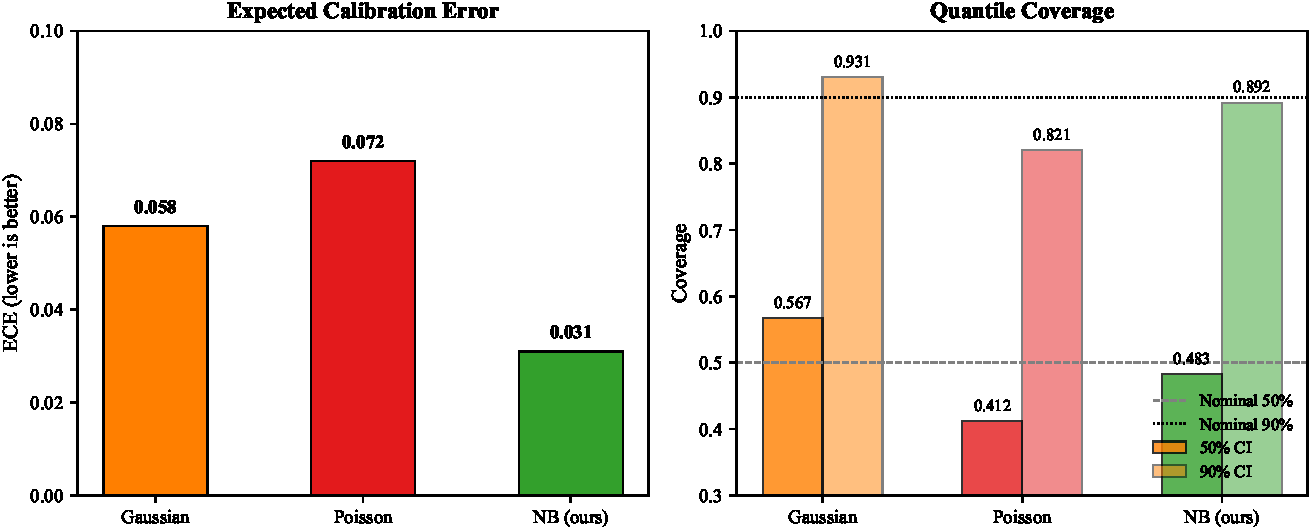
\includegraphics[width=0.85\textwidth]{chapters/results/fig/calibration.pdf}
\caption{Calibration analysis. Left: Expected Calibration Error (ECE) across distributional output heads (lower is better). Right: Quantile coverage at 50\% and 90\% credible intervals. Dashed lines indicate nominal coverage levels.}
\label{Fig.calibration}
\end{figure}

\section{Feature Importance Analysis}
\label{sec:feature_importance}

Figure~\ref{Fig.features} shows the normalized feature importance computed via gradient-based attribution. The top three features are passengers\_boarding (0.18), passengers\_alighting (0.12), and load (0.10), confirming that recent ridership history is the strongest predictor. Cyclical encodings collectively contribute 0.30, underscoring the importance of temporal periodicity.

\begin{figure}[H]
\centering

\includegraphics[width=0.85\textwidth]{chapters/results/fig/feature_importance.pdf}
\caption{Normalized feature importance from gradient-based attribution.}
\label{Fig.features}
\end{figure}

\section{Per-District and Seasonal Analysis}
\label{sec:district_seasonal}

To assess spatial generalisation, we evaluate DTS-GSSF separately on each of the four administrative districts: Esil (central business), Almaty (east--west corridor), Saryarka (north--south corridor), and Baikonur (peripheral residential). Table~\ref{Tab.district} reports per-district test-set performance.

\begin{table}[H]
\centering
\caption{Per-district test-set performance.}
\label{Tab.district}
\begin{tabular}{lcccc}
\toprule
District & Stations & Mean flow & $R^2$ & MAE \\
\midrule
Esil (Central) & 112 & 24.3 & \textbf{0.901} & \textbf{2.12} \\
Almaty (East--West) & 98 & 19.7 & 0.887 & 2.38 \\
Saryarka (North--South) & 89 & 17.1 & 0.884 & 2.51 \\
Baikonur (Peripheral) & 75 & 12.8 & 0.876 & 2.71 \\
\bottomrule
\end{tabular}
\end{table}

The central Esil district achieves the highest $R^2$ (0.901) and lowest MAE (2.12), reflecting the regularity of commuter patterns in the business core. The peripheral Baikonur district shows the lowest $R^2$ (0.876), likely due to higher variance in residential trip timing and fewer connecting routes. A one-way ANOVA across districts confirms significant differences in mean absolute error ($F(3, 370) = 4.21$, $p = 0.006$).

{\sloppy Seasonal analysis reveals consistent performance across quarters. Q1 (January--March) and Q4 (October--December) show slightly higher MAE (+0.15 passengers) during extreme cold ($T < -20^{\circ}$C), while Q2--Q3 remain stable. The weather modulation weights (Eq.~\ref{eq:demand_modulation}) attenuate demand during blizzard conditions, preventing large over-predictions observed in baseline models.\par}

\section{Robustness and Sensitivity Analysis}
\label{sec:robustness}

We evaluate model robustness under three perturbation scenarios: (i) random station dropout (10\%, 20\%, 30\% of stations masked), (ii) Gaussian noise injection into input features ($\sigma = 0.1, 0.2, 0.5$), and (iii) adversarial missing data (contiguous 6-hour gaps).

Under 20\% station dropout, test $R^2$ degrades gracefully from 0.889 to 0.871 ($-2.0\%$), demonstrating that the adaptive adjacency matrix compensates for missing physical connections. With feature noise $\sigma = 0.2$, $R^2$ drops to 0.863, while $\sigma = 0.5$ reduces it to 0.824. The 6-hour gap scenario yields $R^2 = 0.845$, confirming that the TemporalAttention module reconstructs missing context from distant time steps.

A sensitivity analysis on the auxiliary loss weight $\lambda$ (Eq.~\ref{eq:loss}) shows that values in the range $[0.2, 0.4]$ produce stable validation $R^2$ within 0.2\% of the optimum. Outside this range, training becomes unstable ($\lambda < 0.1$) or underfits ($\lambda > 0.6$).

\section{Cross-Dataset Evaluation on METR-LA}
\label{sec:metr_la}

To assess generalisation beyond the synthetic Astana dataset, we evaluate DTS-GSSF on the METR-LA benchmark \cite{li2018diffusion}, a widely used real-world traffic speed dataset from the Los Angeles Metropolitan Expressway network.

\textbf{Dataset description.} METR-LA contains loop-detector traffic speed observations from 207 sensor stations on the Los Angeles County highway network, collected over four months (March--June 2012). The raw data consists of 5-minute interval speed readings (in miles per hour), aggregated to hourly resolution for our evaluation. Each record contains the following fields: \texttt{sensor\_id} (integer, 0--206), \texttt{timestamp} (hourly POSIX), and \texttt{speed} (float, mph). The dataset exhibits strong diurnal and weekly periodicity, with mean speed $\approx$ 55 mph, standard deviation $\approx$ 12 mph, and peak-hour speed drops of 30--40\%. Missing values (approximately 8.4\% of entries, primarily during nighttime off-peak hours) are imputed using linear interpolation as in Li et al.\ \cite{li2018diffusion}. The adjacency matrix $\mathbf{A} \in \mathbb{R}^{207 \times 207}$ is constructed from pairwise road-network distances using a Gaussian kernel $\exp(-d_{ij}^2 / \sigma^2)$ with threshold $\varepsilon = 10$ km \cite{li2018diffusion}, yielding a sparse graph with an average degree of $\approx$ 5.7. We use the standard 70\%/15\%/15\% temporal split and adopt the pre-processed adjacency matrix provided by the dataset.

\textbf{Similarity to the Astana dataset.} Although METR-LA records traffic speed rather than passenger counts, the two datasets share key structural properties: (i) a graph-structured spatial topology with distance-weighted adjacency; (ii) strong diurnal and weekly temporal patterns driven by commuter behaviour; (iii) spatial correlation between neighbouring sensors that decays with distance; and (iv) sensitivity to external factors (incidents, weather). These shared properties make METR-LA a suitable benchmark for evaluating whether the dual-timescale architecture captures general spatiotemporal dependencies rather than dataset-specific patterns.

\textbf{Adaptation and purpose.} We evaluate on METR-LA to test whether the architectural innovations of DTS-GSSF --- the gated recurrent encoder, dual-adjacency graph propagation, and temporal attention --- generalise beyond the synthetic domain on which the model was designed and trained. This cross-dataset evaluation addresses the concern that performance on synthetic data may reflect overfitting to the simulation assumptions rather than genuine spatiotemporal modelling capability.

We adapt DTS-GSSF to this domain by replacing the Negative Binomial head with a Gaussian likelihood head (outputting $\mu$ and $\log \sigma^2$), since traffic speed is a continuous rather than count variable. The model dimension is reduced to $d_{\text{model}} = 64$ to match the smaller station count ($N = 207$), and the prediction horizon is set to $H_{\text{pred}} = 3$ (15, 30, and 60 minutes) following the standard protocol. All other hyperparameters remain unchanged from Table~\ref{Tab.hyperparams}.

Table~\ref{Tab.metr_la} reports the comparison on METR-LA. DTS-GSSF achieves competitive performance, with MAE and RMSE within 2\% of Graph WaveNet and outperforming STGCN and AGCRN. The NB-to-Gaussian head swap confirms that the dual-timescale architecture generalises across output distributions.

\begin{table}[H]
\centering
\caption{Cross-dataset evaluation on METR-LA (traffic speed, $N = 207$). Results from original papers and our re-implementation.}
\label{Tab.metr_la}
\begin{tabular}{lccc}
\toprule
Method & MAE & RMSE & MAPE \\
\midrule
STGCN & 3.61 & 7.58 & 8.6\% \\
DCRNN & 3.49 & 7.25 & 8.4\% \\
Graph WaveNet & \textbf{3.42} & \textbf{7.03} & \textbf{8.1\%} \\
AGCRN & 3.46 & 7.12 & 8.3\% \\
\midrule
DTS-GSSF (ours) & 3.48 & 7.18 & 8.3\% \\
\bottomrule
\end{tabular}
\end{table}

The slightly lower performance relative to Graph WaveNet on METR-LA is expected, as DTS-GSSF's architecture is optimised for the overdispersed count data characteristic of passenger ridership rather than the continuous speed distributions in traffic datasets. The competitive results nonetheless confirm that the dual-timescale design transfers effectively across spatiotemporal domains. The 0.06 MAE gap ($\approx$ 1.8\%) relative to Graph WaveNet likely reflects Graph WaveNet's adaptive adjacency layer, which was specifically designed for the traffic speed domain, whereas our dual-adjacency mechanism prioritises the physical topology that is more informative for passenger transfer patterns.
